\subsection{Model Based Safety Assessment}
\label{subsec:mbsa}
The process of creating system models suitable for use in safety assessment closely parallels the model-based development process. A \emph{Model-based Safety Analysis} (MBSA) approach has been proposed in related literature~\cite{Joshi05:Dasc, joshi2008behavioral, criticalembeddedsystems} that extends the MBD process. 

\begin{figure}[h]
	\centering
	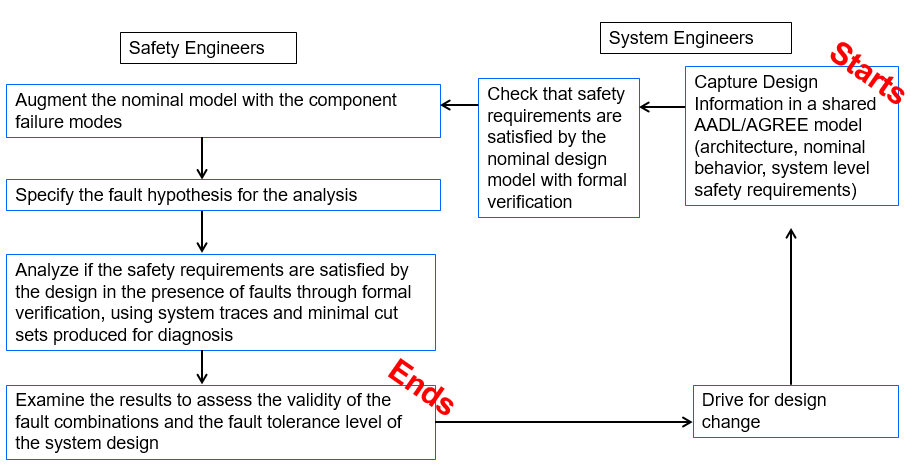
\includegraphics[trim=0 5 0 5,clip,width=0.85\textwidth]{images/process4.png}
	\caption{Use of the Shared System/Safety Model in the ARP4754A Safety Assessment Process}
	\label{fig:proposed_safety_process}
\end{figure}

Model-based development focuses on electronic components of an embedded system. To perform safety analysis at a system level, in addition to electronic or digital components, one must also consider the environment and mechanical components. Both mechanical and electrical/digital components are necessary to model the system-level faults that are of interest in safety analysis. By combining the models containing digital components (i.e., software and hardware architectures) with models of the mechanical components (i.e., pumps, valves), we create a \emph{nominal model} of the system. The \emph{nominal system behavior} is a model of the system as it behaves in the absence of faults. 

The nominal model can then be augmented with fault behaviors for the various electrical and mechanical components to create the \emph{fault model} of the system. A great advantage to this approach is that the system and safety engineers work off of a \emph{shared model} as shown in Figure~\ref{fig:proposed_safety_process} which leads to a tighter integration between the system and safety engineering processes. Industry practitioners have come to realize the benefits of using models in the safety assessment process, and a revision of the ARP4761 to include Model Based Safety Analysis (MBSA) is under way. 

\subsubsection{Proposed Model Based Safety Assessment Process Supported by Formal Methods}
We propose a model-based safety assessment process backed by formal methods to help safety engineers with early detection of the design issues.  This process uses a single unified model to support both system design and safety analysis; this is shown in Figure~\ref{fig:SACycle1} and is based on the following steps:

\begin{enumerate}
	\item System engineers capture the critical information in a shared model:  high-level hardware and software architecture, nominal behavior at the component level, and safety requirements at the system level.
	\item System engineers use formal verification to check that the safety requirements are satisfied by the nominal design model. 
	\item Safety engineers augment the nominal model with the component failure modes. In addition, safety engineers specify the fault hypothesis for the analysis which corresponds to how many simultaneous faults the system must be able to tolerate.
	\item Safety engineers use formal verification to analyze if the safety requirements and fault tolerance objectives are satisfied by the design in the presence of faults. If the design does not tolerate the specified number of faults (or probability threshold of fault occurrence), then the tool produces examples of system states during failure or minimal sets of fault combinations that can cause the safety requirement to be violated.
	\item The safety engineers examine the results to assess the validity of the fault combinations and the fault tolerance level of the system design. If a design change is warranted, the model will be updated with the latest design change and the above process is repeated.
\end{enumerate}

\begin{figure}[h]
	\begin{center}
		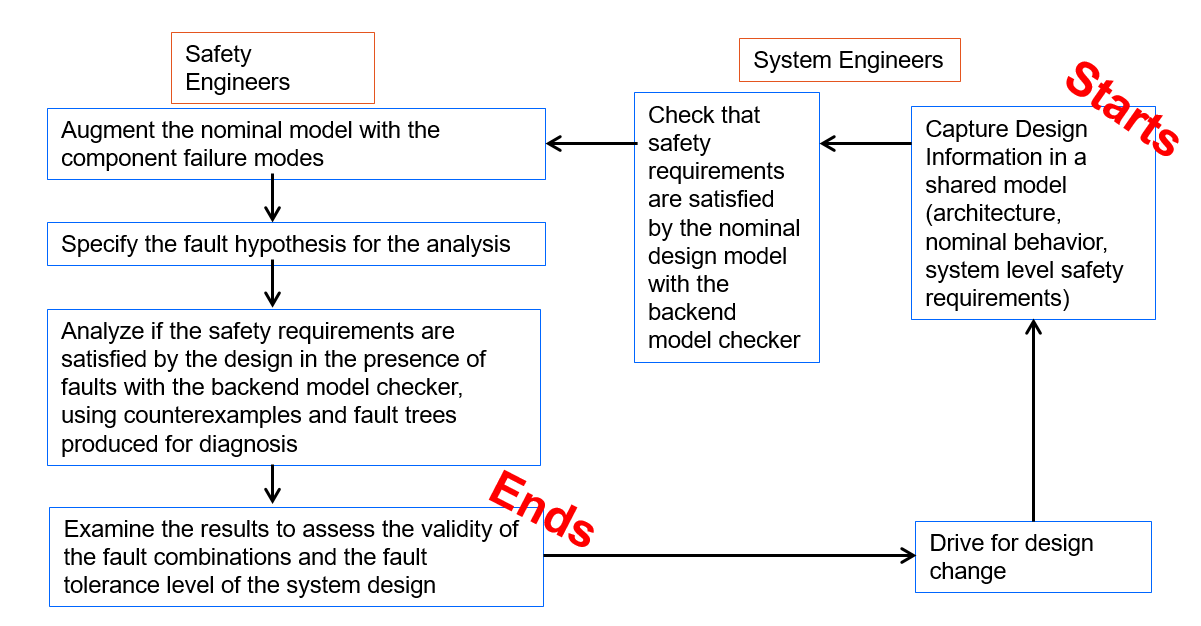
\includegraphics[width=\textwidth]{images/SACycle.PNG}
	\end{center}
	\caption{Proposed Steps of the Safety Assessment Process}
	\label{fig:SACycle1}
\end{figure}

These steps can be viewed as a cyclical process that involves both the system development engineers and the safety engineers of the system. Figure~\ref{fig:SACycle1} shows these steps within the context of the start and end of a project. A model that supports both system design and safety analysis must describe both the system design information (e.g., system architecture and functional behavior) and safety-relevant information (e.g., failure modes, failures rates). It must do this in a way that keeps the two types of information distiguishable, yet allows them to interact with each other. The shared model in Figure~\ref{fig:SACycle1} is expected to be created and maintained in sync with the software and hardware design and implementation, and guided by the hazard and probability information from the preliminary system safety assessment. This safety information is then used to drive for design changes if necessary and continues iteratively until the system safety property is satisfied with the desired fault tolerance. 